%Technology: precise description of the technology / approach that is used

% Inspiré de la section 10 du papier formose

\begin{figure}[t]
    \centering
    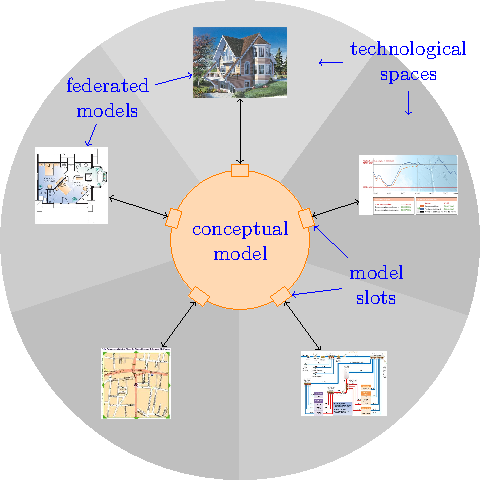
\includegraphics[width=\columnwidth]{Figures/federation.pdf}
    \caption{The model federation approach}
    \label{fig:mf}
\end{figure}

To meet the \mlpc, we have decided to use the language infrastructure of
model federation approach~\parencite{Golra2016-federation}. \emph{Model
  federation} is a way to assemble models using some kind of
low-coupling links. It was initially  formulated to respond to the \OMG's RFP
Semantic Modeling for Information Federation~\parencite{simf}. In
contrast to approaches that compose metamodels into a single large
metamodel grouping all needed entities, model federation build links
between models and metamodels (even through levels) to make ``things''
work together. As an illustration of this feature, we developed a
free-modeling editor -- freeing oneself from the bonds of
model/metamodel conformity -- that is presented
in~\parencite{models2016-freemodel}. Another notable feature of
this approach is the strong decoupling among tools that remain usable
after federations are made.
So to provide an adaptable framework, we have developed a flexible modeling language to provide modeling features without strict modeling levels. In a federation, the targeted modeling approaches can be unknown at the beginning and also can integrate several modeling levels.


We decided to use this approach since it offers the possibility to
link and to navigate among levels. Before we describe the 
architecture in next section, here are some key concepts implemented
in the Openflexo~\parencite{openflexo_link} framework.

% figure
% Dans la suite les références à la figure sont commentés


\begin{figure*}
    \centering
    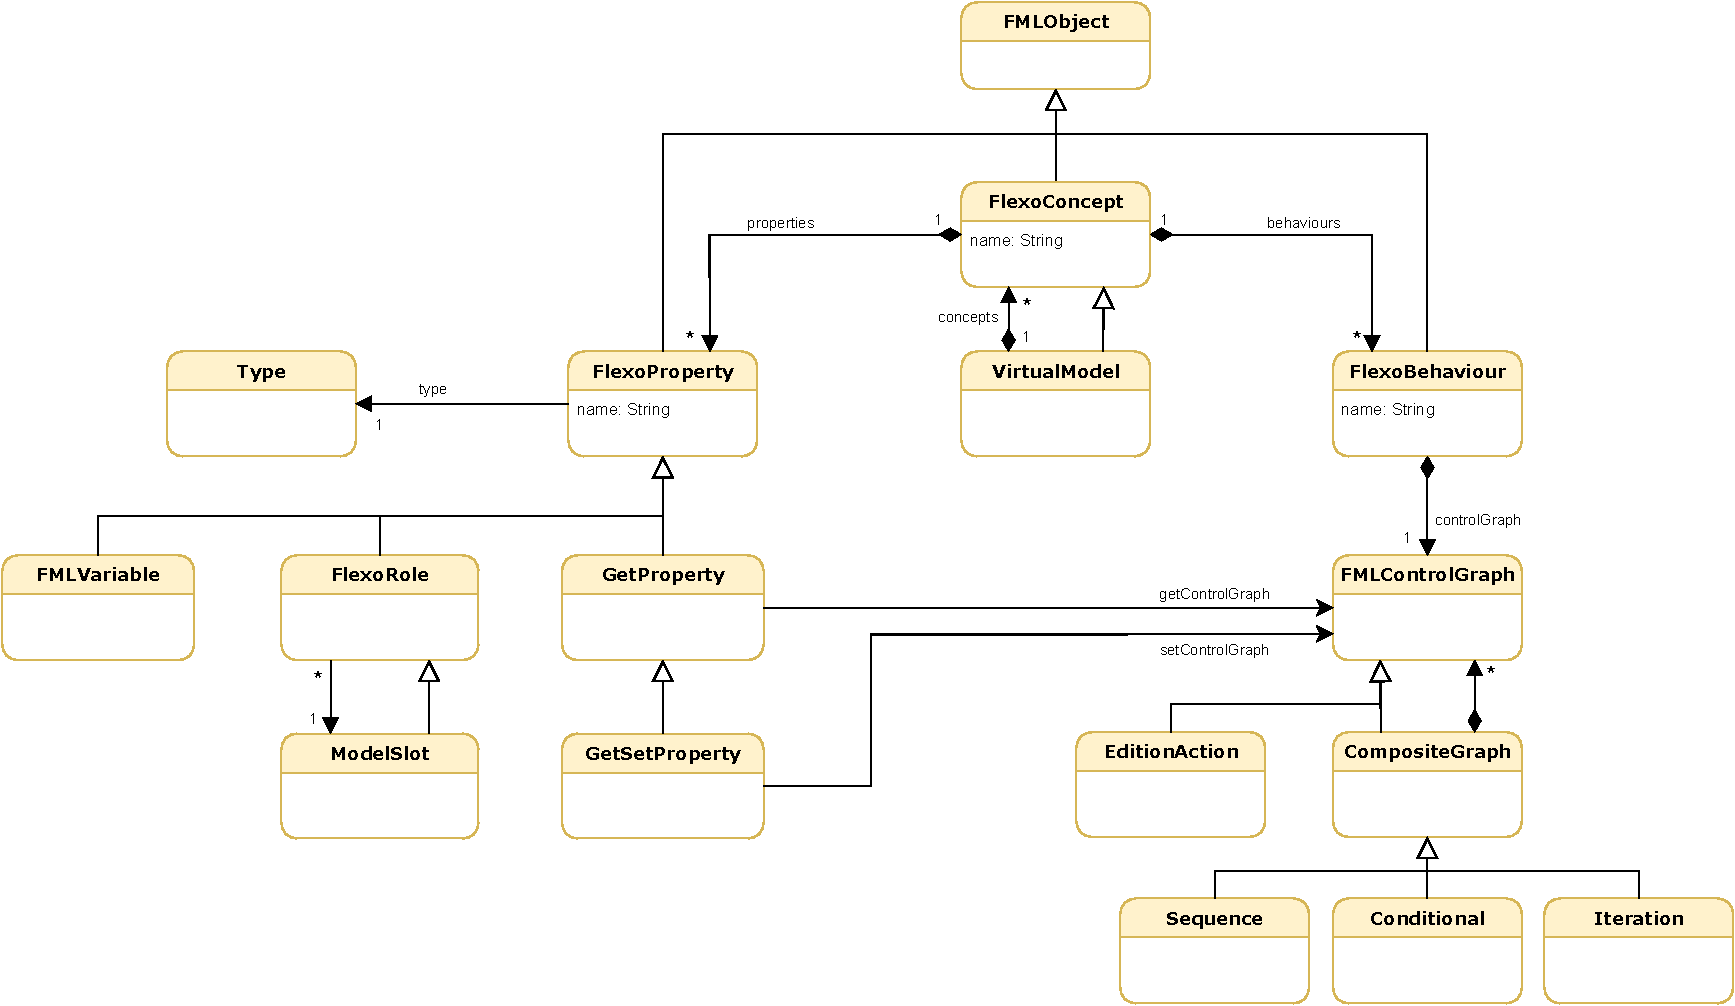
\includegraphics[width=1.0 \textwidth]{Figures/FMLMetaModel-1.5.pdf}
    \caption{Representation of the main concepts of {FML} language}
    \label{fig:mm}
\end{figure*}
%\noteAntoine{Dans la figure ne manque-t-il pas les containements ? (VM vers Concepts)}
%\noteSylvain{C'est le cas dans cette nouvelle figure}

This framework relies on the architecture of Fig.~\ref{fig:mf}. A federation
gathers a set of conceptual models, named \emph{virtual models} and a
set of \emph{federated models}. Each federated model pertains to a
\emph{technological space} and uses the language of its specific
paradigm while a virtual model is built using the Federation Modeling
Language (\FML). Each federated model is an autonomous
element that may evolve with its own tooling {\color{red} tooling is used in place of tool throughout the article.  I suggest clarifying it and then editing it all along the article}. The virtual models
serve as control elements binding the federated models together.
In this paper, we mainly use conceptual models and more precisely \FML, its domain specific modeling language. The only use of the federation aspect is on the tooling made for the process language.

{\color{red} This paragraph needs a parallel in naming convention between Figure 2 and the text.  FlexoConcept, FlexoBehavior, etc.} A \UML like representation of a simplified metamodel of \FML is provided in Fig.~\ref{fig:mm}. \FML is a language designed to define virtual models. A \emph{virtual model} is composed of a set of \emph{concepts}, while itself being a \emph{concept}. Hence, \emph{virtual models} are structuring units forming architectures while \emph{concepts} are the core entities. A concept has a set of \emph{properties} and \emph{behaviors}. \emph{Properties} can be either simple variables, roles (pointers to a modeling element in a \emph{virtual model} or an external technology-specific model), or properties bound to complex control graphs. \FML is designed to define not only the structure of virtual models but also the collection of actions that can be performed on them. These actions are called \emph{behaviors} and rely on behavioral primitives called \textsf{EditionAction}. These \emph{behaviors} can either be called or triggered by events. The reactive behaviors are useful when a federated model evolution needs to trigger a computation. Note that we do not exploit this possibility in the challenge.

A parallel to object-oriented approach can be useful to understand \FML\footnote{Some aspects of \FML do not exist in object oriented approach.}. A concept corresponds to a class, its properties to the attributes of the class and its behaviors to the methods of the class. These properties have types defining the kind of value the role will point at runtime. Whenever an element external to the federation space is used, one needs to use a \emph{model slot}. A model slot is a mediation entity in charge of giving access to external elements using a \emph{technology adapter}\footnote{It is a reusable library that defines connections between the \FML execution engine and a particular technological space.}.

When the \FML execution engine runs a federation, it creates virtual
model instances containing concept instances. Some concept instances
are connected to external elements through model slot instances.

% Sylvain : relire et vérifier


\begin{figure}[t]
    \centering
    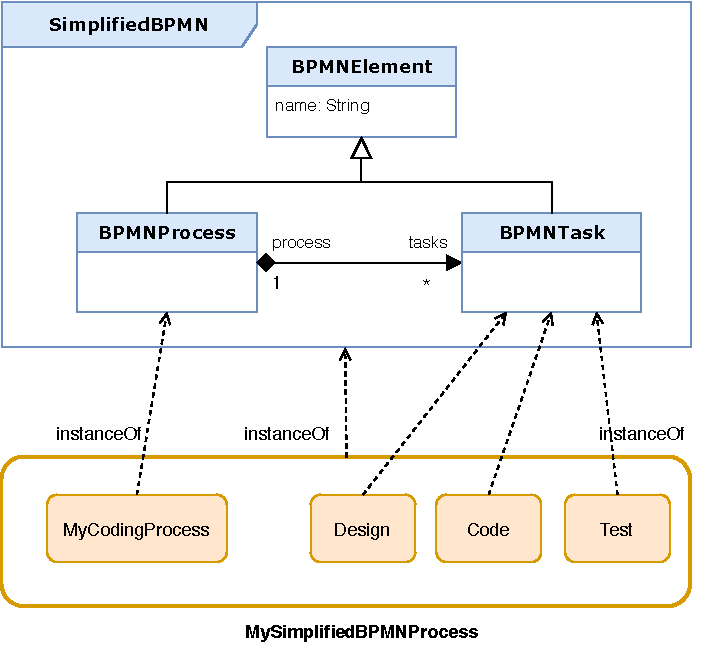
\includegraphics[width=\columnwidth]{Figures/BPMNSubsetExample-1.5.pdf}
    \caption{An example of \BPMN subset showing both the model and an instance of that model}
    \label{fig:BPMNSubsetExample}
\end{figure}

To illustrate this, Fig.~\ref{fig:BPMNSubsetExample} shows how to realize a
small subset of \BPMN with Openflexo/FML. Concretely, we have designed a \textit{virtual model} (\texttt{SimplifiedBPMN}) with 3 \textit{concepts} representing a process and its contained tasks. An instance of this \textit{virtual model} is presented in the bottom of the figure, showing instances with their \textsf{instanceOf} relationships with their model.
%
The following listing shows the \FML code of this \textit{virtual model}. Note that the composition relation of Fig.~\ref{fig:BPMNSubsetExample} between \texttt{BPMNProcess} and \texttt{BPMNTask} is realized in the FML code by concept containment. Whenever an instance of \texttt{BPMNTask} is created, it must be in a container (instance of \texttt{BPMNProcess}) and the two instances get linked together. %\noteFabien{A valider}

\begin{lstlisting}
// A simplified BPMN metamodel exposing the
// concepts BPMNProcess and BPMNTask
model SimplifiedBPMN {

  // Abstract concept BPMNElement defining a name
  abstract concept BPMNElement {
    String name;
    // A basic constructor
    create(String name) { this.name = name; }
  }

  concept BPMNProcess extends BPMNElement {

    // A basic constructor
    create(String name) { super(name); }
    // Other properties and behaviours of the
    // BPMNProcess concept
    ...

    concept BPMNTask extends BPMNElement {

      // A basic constructor
      create(String name) { super(name); }
      // Encodes execution of task
      execute() {
        log("Execute task "+name);
        ...
      }
      // Other properties and behaviours of the
      // BPMNTask concept
      ...

    }

    // Other concepts
  }
}
\end{lstlisting}

%\noteSylvain{A la fin de la rédaction, s'arranger pour que la figure 3 (fig:BPMNSubsetExample) et le listing soient cote a cote, et aussi que le listing tienne sur une seule page}

The tool support for model federation framework,
Openflexo\footnote{\url{https://github.com/openflexo-team}}, is
developed as an open source initiative. This tool offers an \FML
execution engine with an interactive virtual model design environment.

Finally, tools have their own model. We have taken advantage of Openflexo features to build, in addition to the models  required by the challenge, a drawing tool that makes our
solution (partially) executable.
